\chapter{Chapitre 5 : Algorithmes des éléphants pour le problème de recherche de cibles}

\label{Chapter5}

\section{Introduction}
La deuxième contribution majeure de ce projet est l'adaptation des deux algorithmes basés
essaim d'éléphants vus précédemment, à savoir EHO et ESWSA pour le problème de la
recherche de cibles.
Il sera question dans ce chapitre d'effectuer une adaptation de l'ensemble des concepts de ces deux méthodes de résolution à la modélisation exhibée au niveau du chapitre 3, ainsi que les différentes étapes de leur fonctionnement. 


\section{Adaptation de EHO pour le problème de la recherche de cibles}
L'algorithme EHO fut présenté de manière générale au niveau du chapitre 2, nous allons maintenant nous intéresser à son adaptation au problème de recherche de cibles. Les aspects phares de cette approche seront redéfinies comme suit :


\subsection{Solution}
Une solution est la position de coordonnées \textit{(x, y)} dans laquelle se trouve un éléphant.

\subsection{Fonction objectif}
La fonction objectif est comme définie pour l'approche BSO, à la différence près que pour EHO ce sont les éléphants qui sont responsables de l'évaluation des solutions.


\subsection{Éléphant}
Un éléphant est un robot, il occupe une case unique dans l'environnement à chaque instant \textit{"t"}. La mise à jour de la position d'un éléphant par rapport à son clan suit l'équation \ref{eq:xnew} pour les deux dimensions \textit{(x,y)}, comme suit :
\begin{equation}
\begin{split}
{x}_{new,c,i} = {x}_{c,i} + \alpha *( {x}_{Best,c} - {x}_{c, i} ) * r \\
{y}_{new,c,i} = {y}_{c,i} + \alpha *( {y}_{Best,c} - {y}_{c, i} ) * r 
\end{split}
\end{equation}

La figure \ref{elephant} ci-dessous représente l'influence de la meilleure solution sur le déplacement des autres éléphants du clan selon différents degrés $\alpha$.
\begin{center}	  
	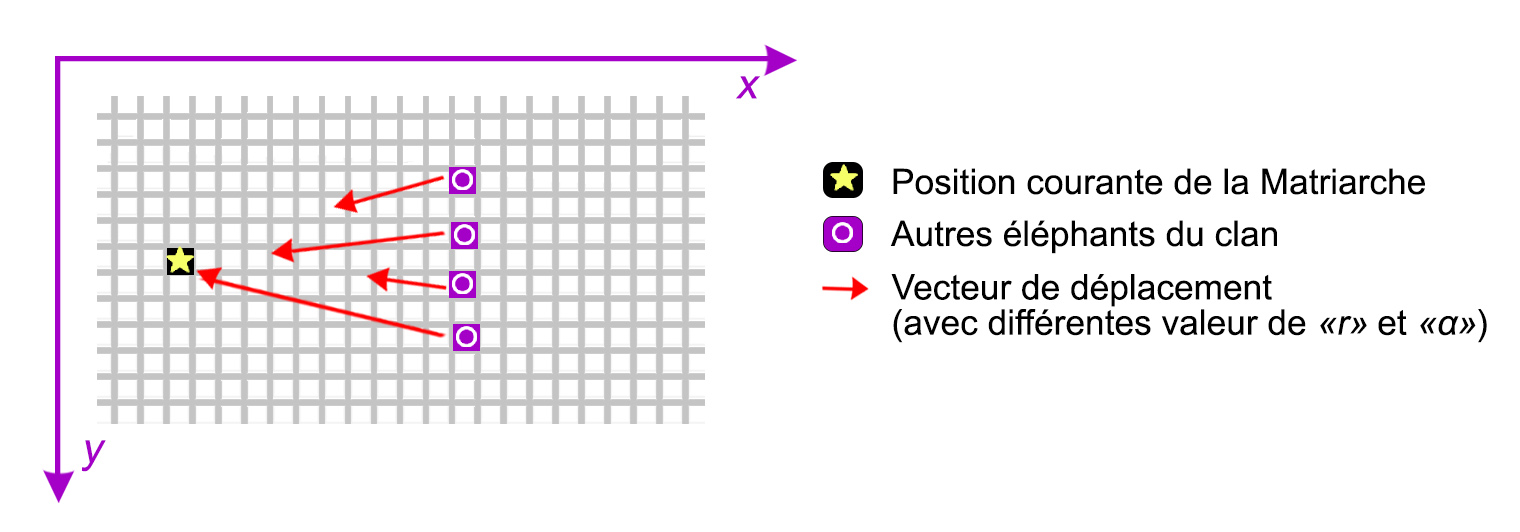
\includegraphics[width=0.9\textwidth]{elephant.jpg}%
	\vspace{-0.3cm}
	\captionof{figure}{Représentation de la méthode de mise à jour des positions des éléphants.}\label{elephant}%
\end{center}

\subsection{Clan}
\label{clanArea}
Les éléphants d'un même clan sont généralement regroupés dans une même zone. Ainsi, les positions initiales des éléphants sont générées comme suit:
\begin{enumerate}
	\item Pour chaque clan générer une position initiale aléatoirement.
	\item À partir de chaque position générée, positionner les \textbf{nbrElephant} - 1 autres éléphants sur une surface ronde de rayon inférieur ou égale à une certaine limite (5 cases dans notre cas).
\end{enumerate}
La figure \ref{clan} ci-dessous, représente un exemple de positions générées pour les éléphants d'un même clan :
\begin{center}	  
	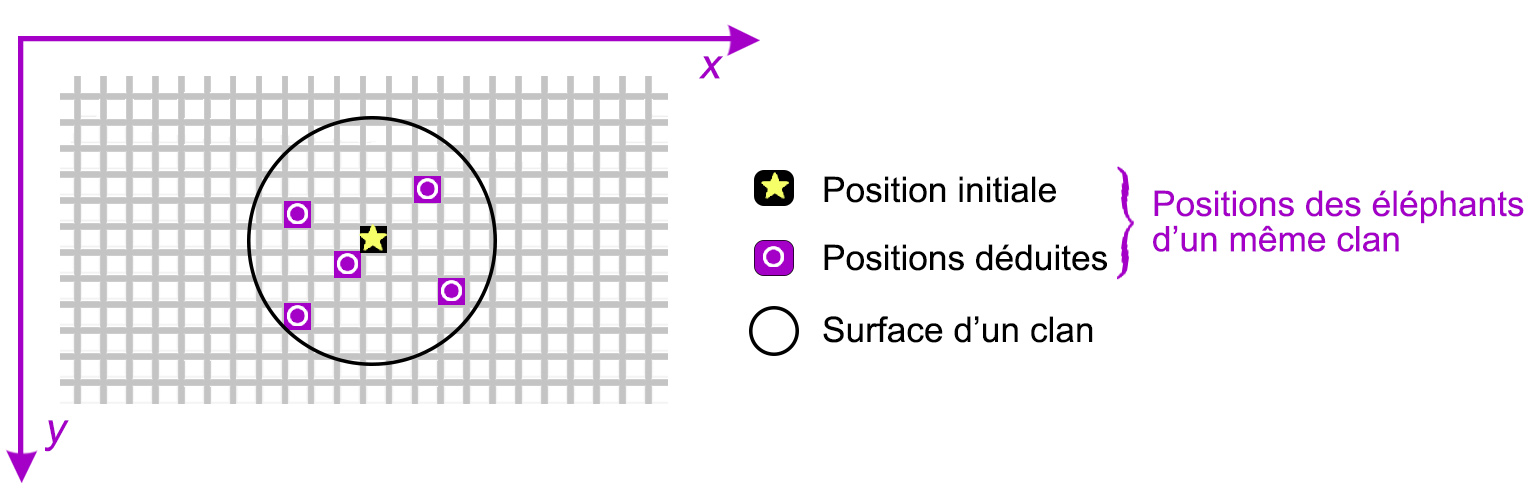
\includegraphics[width=0.95\textwidth]{Clan.jpg}%
	\vspace{-0.1 cm}
	\captionof{figure}{Représentation de la technique de génération des positions des éléphants d'un même clan.}\label{clan}%
\end{center}

\subsection{Chef de clan (Matriarche) }
L'éléphant chef de clan appelé "Matriarche" est celui qui possède la meilleure solution de son clan. La mise à jour de cette position dépend du centre de gravité du clan, comme présentée dans l'équation \ref{eq:xbest}, elle est appliquée de la même manière à chacune des coordonnées \textit{x} et \textit{y}, comme suit :
\begin{equation}
\begin{split}
{x}_{Best,c} = \beta  *  {x}_{center,c} \\
{y}_{Best,c} = \beta  *  {y}_{center,c}  
\end{split}
\end{equation}

De même, le centre de gravité est calculé pour les deux dimensions, par l'équation:
\begin{equation}
	\begin{split}
	{x}_{center,c}  = \frac{1}{N} * \sum_{i=1}^{N} {x}_{c,i}\\
	{y}_{center,c}  = \frac{1}{N} * \sum_{i=1}^{N} {y}_{c,i}
	\end{split}
\end{equation}

La figure \ref{chef} montre le processus de mise à jour de la position de la "Matriarche".

\begin{center}	  
	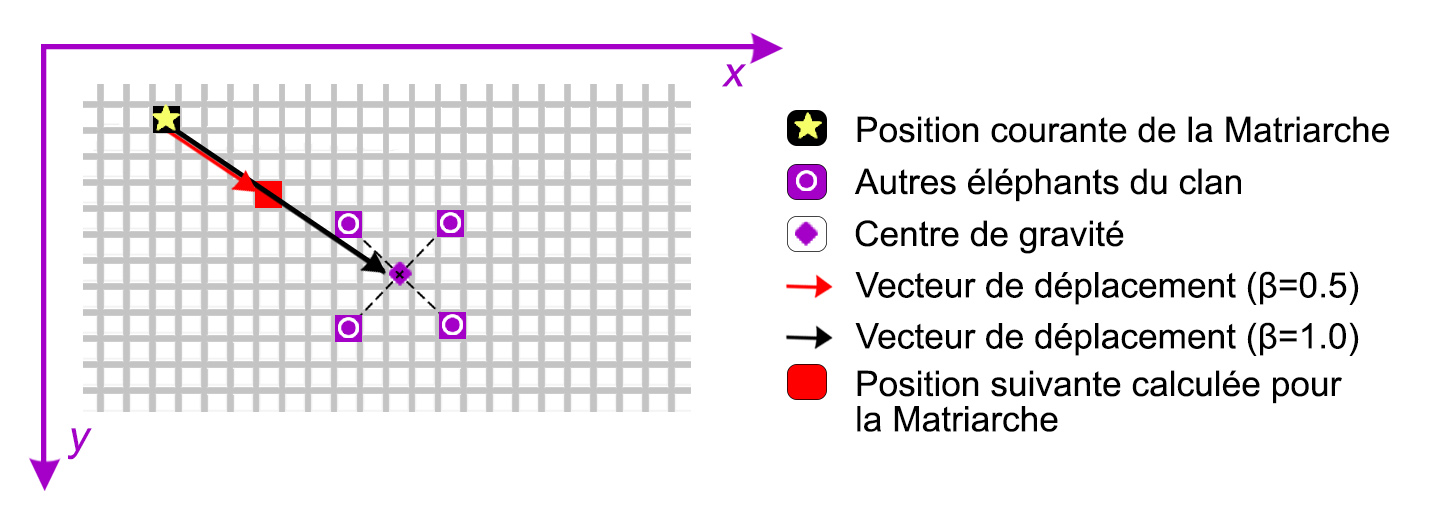
\includegraphics[width=0.95\textwidth]{chefClan.jpg}%
	\vspace{-0.1 cm}
	\captionof{figure}{Représentation de la méthode de mise à jour de la position du meilleur éléphant/robot.}\label{chef}%
\end{center}

\subsection{Éléphant mâle}
Dans chaque clan, l'éléphant évalué comme détenant la pire solution est appelé \textit{"pire éléphant"}. Il possède une fonction de mise à jour particulière décrite par l'équation \ref{eq:xworst}, qui pour notre environnement 2D de taille $taille_{Coté}$ est adaptée par l'équation :
\begin{equation}
\begin{split}
{x}_{Worst,c}  =  (taille_{Cot\acute{e}} - 1) * rand \\
{y}_{Worst,c}  =  (taille_{Cot\acute{e}} - 1) * rand 
\end{split}
\end{equation}

Celle-ci favorise la diversification afin d'explorer une plus grande surface de l'environnement.
Un exemple d'application de cette équation est présenté dans la figure \ref{worst} qui suit :

\begin{center}	  
	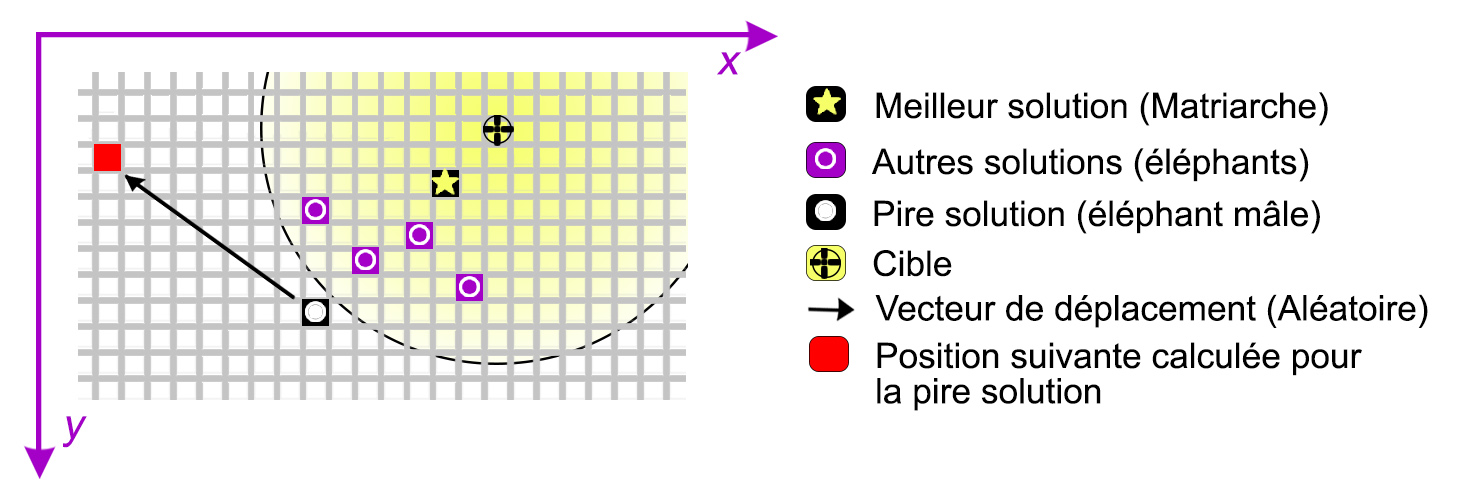
\includegraphics[width=0.95\textwidth]{worst.jpg}%
	\vspace{-0.1 cm}
	\captionof{figure}{Représentation de la méthode de mise à jour de la position du pire éléphant/robot.}\label{worst}%
\end{center}



%\newpage

\section{Fonctionnement d'EHO}
La méthode EHO repose sur la présence de plusieurs clans de robots éléphants, où chaque clan possède un chef aussi appelé \textit{"meilleur éléphant"} ou \textit{"Matriarche"} et un pire éléphant devant se séparer du clan. Les différents clans coopèrent dans le but commun de recherche de cibles. Deux types de communication sont utilisés, d'abord la communication entre robots d'un même clan sur les meilleures solutions trouvées, en second lieu la communication entre clans relative au nombre de cibles, celle-ci faisant office de tableau noir. L'organigramme de la figure \ref{eho} décrit son fonctionnement.

\subsection{Initialisation des positions des clans}
Pour commencer, nous initialisons les positions des \textbf{"nbrClan"} clans de manière aléatoire dans notre espace des solutions, en tenant compte des contraintes concernant les bornes et les obstacles de ce dernier.

\subsection{Initialisation des positions des éléphants}
À partir des positions des clans, sont déduites les positions des \textbf{"nbrEle"} éléphants de chaque clan comme décrit dans la section \ref{clanArea}.



\subsection{Évaluation des solutions }
\label{eval}
Chaque clan \textit{"Cl"} se voit évaluer les solutions que portent tous ses éléphants.
Dès qu'une nouvelle cible est trouvée, le nombre de cibles détectées \textit{"c"} est incrémenté. Ainsi, si le nombre total de cibles \textbf{"nbrCible"} de notre environnement est atteint, la mission de recherche est un succès et donc interrompue.

\subsection{Tri des clans}
Chaque clan parmi les \textbf{"nbrClan"}, procède au tri de ses éléphants selon la fonction objectif dans l'ordre décroissant de ses valeurs.

\subsection{Mise à jour des positions des éléphants}
Pour chaque éléphant \textit{"ele"} du clan \textit{"Cl"} on détermine la nouvelle position. Pour cela, les deux paramètres nécessaires sont la position du chef de clan et le paramètre empirique $\alpha$.\\

La nouvelle position du meilleur éléphant de chaque clan est calculée à partir du centre de gravité du clan $CG_{Cl}$ et du paramètre empirique $\beta$.\\

La génération de la prochaine position du pire éléphant de chaque clan grâce à l'opérateur de séparation de base aléatoire.

\subsection{Déplacement des robots}
Chaque robot éléphant \textit{"ele"} se déplace vers la nouvelle position calculée via notre processus d'évitement d'obstacles.


\subsection{Test de la condition d'arrêt}
Incrémenter le nombre d'itérations effectuées \textit{"t"}.
Le processus de recherche prend fin si le nombre maximum d’itérations \textbf{"MaxIter"} est atteint. Dans le cas contraire, le processus reprend à partir de l'étape d'évaluation des solutions (section \ref{eval}). 
	


\noindent

\begin{center}	  
	\captionsetup{width=1\linewidth}
	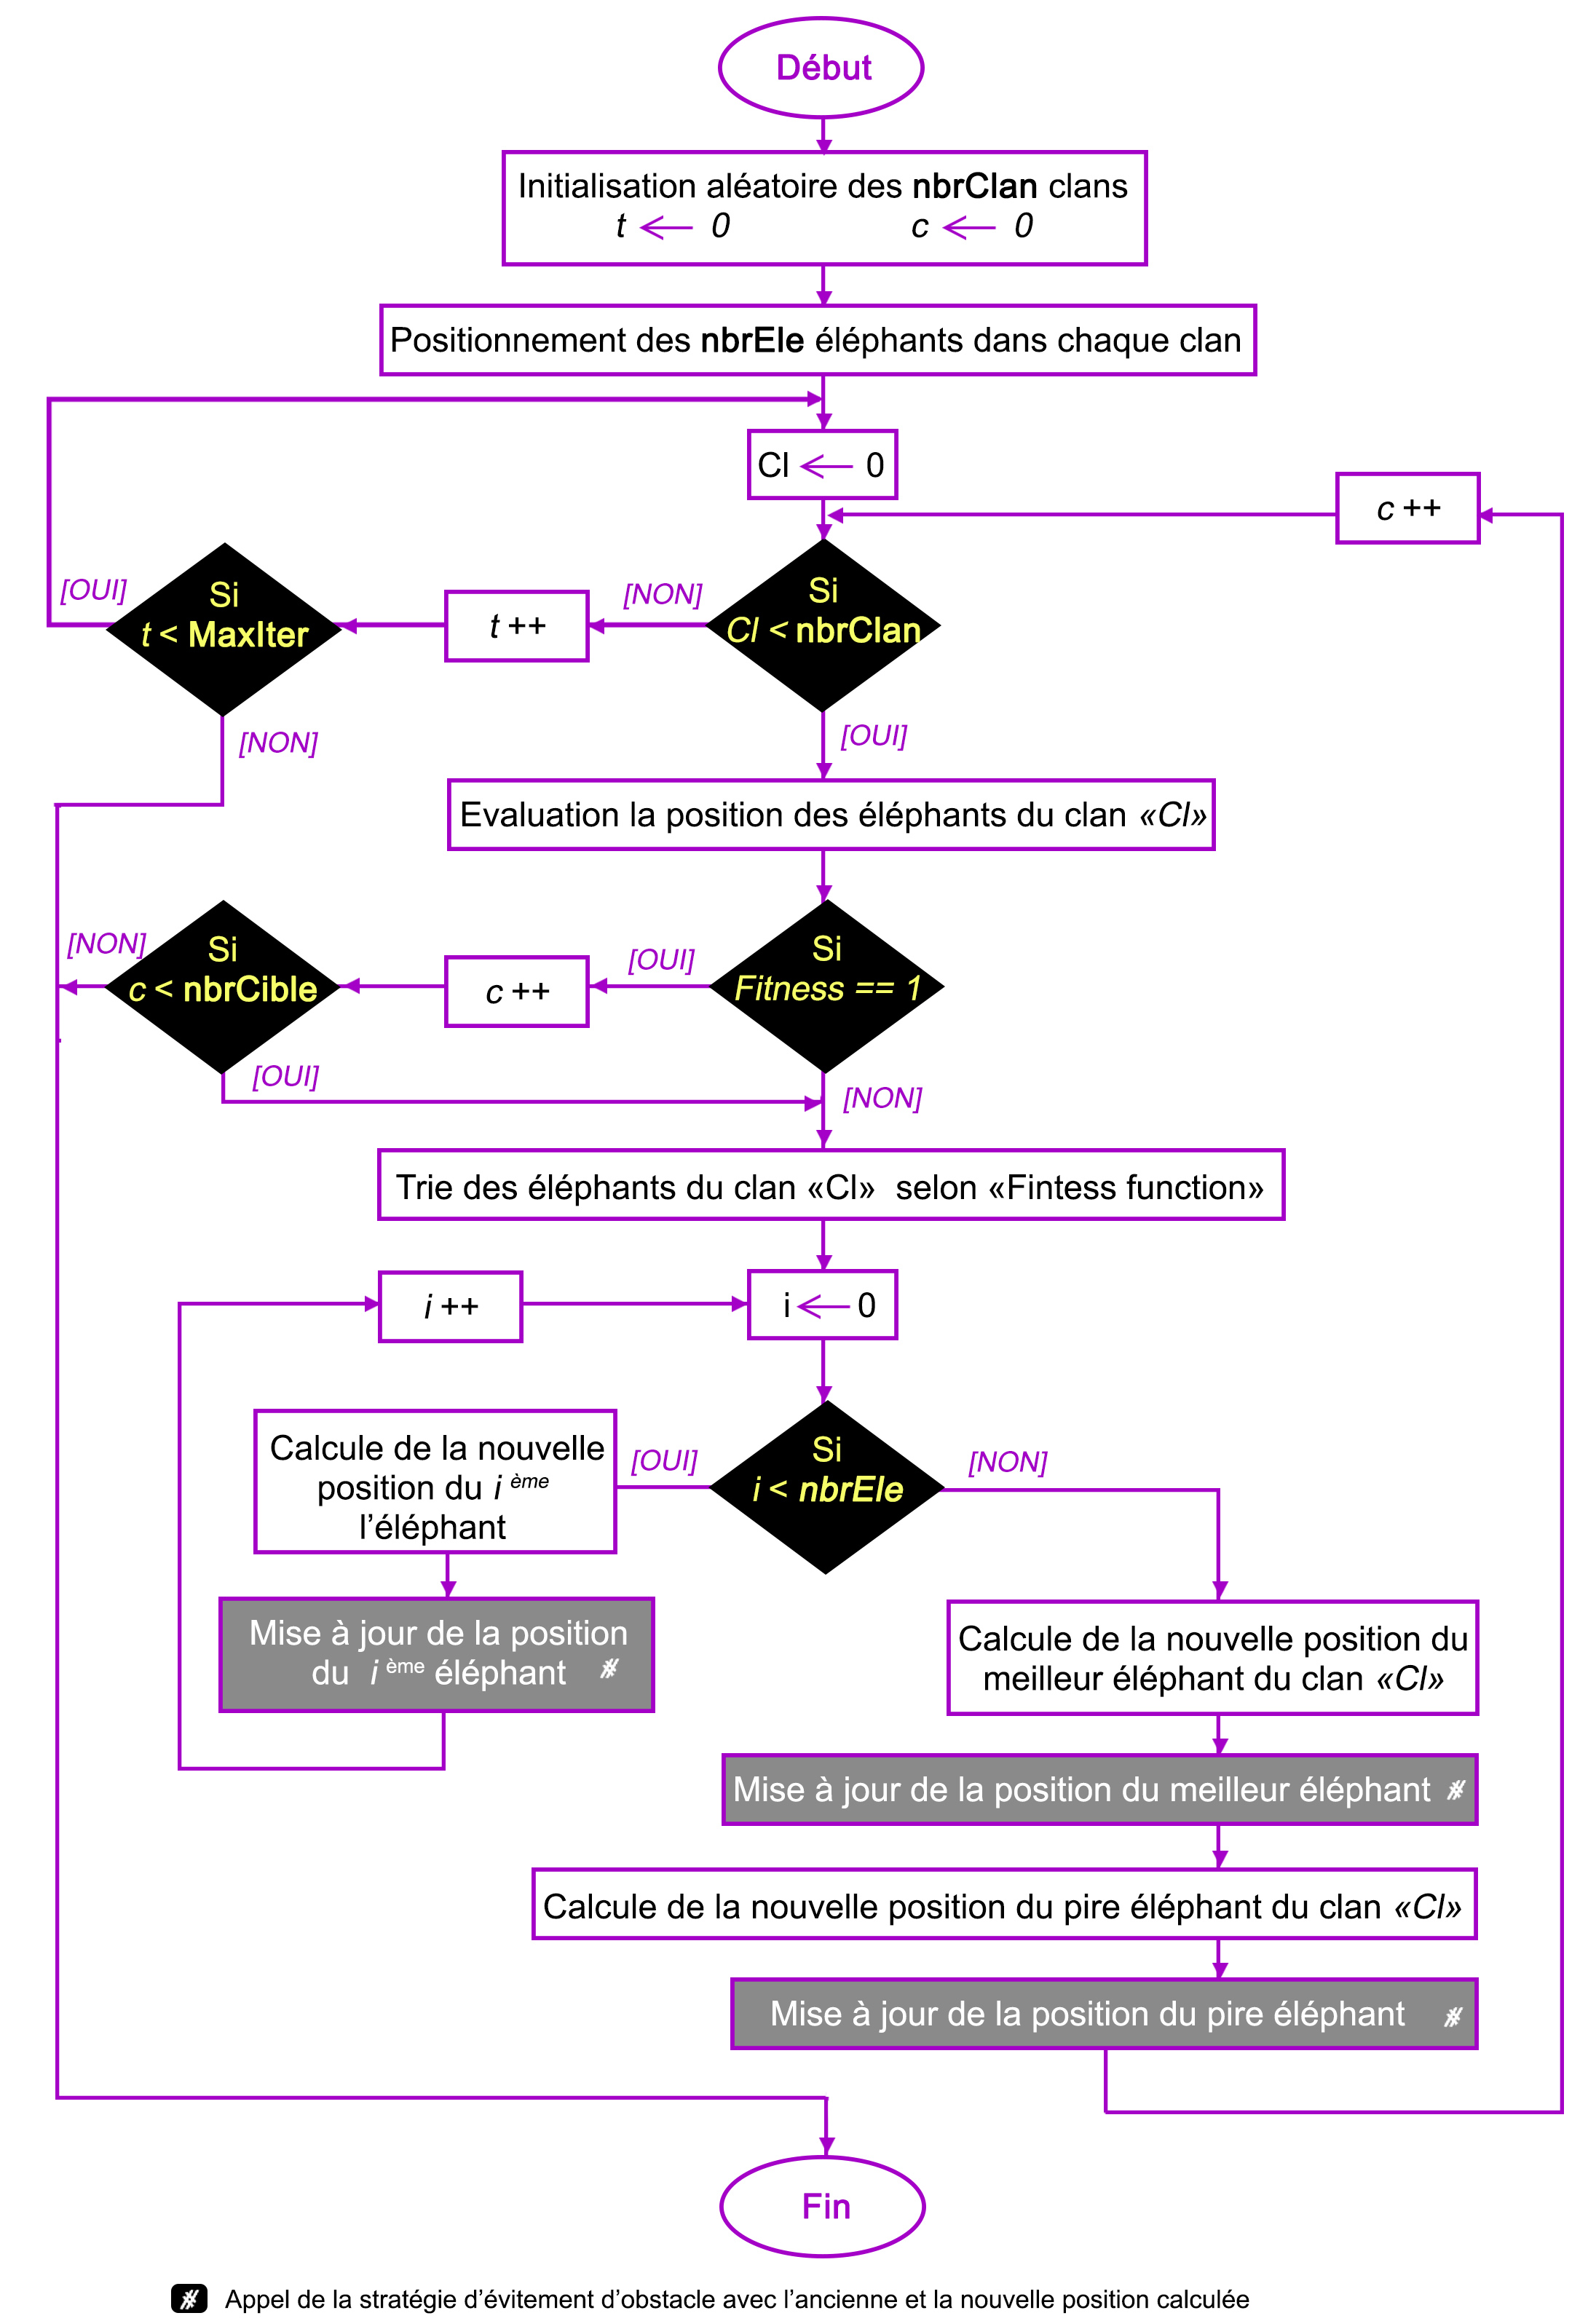
\includegraphics[width=0.95\textwidth]{eho.jpg}%
	\vspace{-0.1 cm}
	\captionof{figure}{Organigramme du mode de fonctionnement de l'approche EHO.}\label{eho}%
\end{center}



\newpage

\section{Adaptation de ESWSA pour le problème de la recherche de cibles}
\subsection{Solution}
Tout comme EHO, une solution pour ESWSA est la position de coordonnées \textit{(x, y)} occupée par un éléphant se comportant comme un robot.

\subsection{Fonction objectif}
La fonction objectif est la même que pour EHO, où les éléphants sont responsables de l'évaluation des solutions.


\subsection{Éléphant}
Un éléphant simule un robot, il occupe une case dans la grille de l'environnement. Il est doté d'une mémoire qui englobe sa meilleure position personnelle "$pbest$" et la meilleure position globale "$gbest$" du groupe d'éléphants.
La dimension du vecteur de positions est alors égale à deux.
\begin{equation}
X_{i,2} = (x_{i1},x_{i2})
\end{equation}
Pour des soucis de compréhension on a choisi la notation $(x,y)$ avec $i$ l'identifiant de l'éléphant
\begin{equation}
X_{i,2} = (x_{i},y_{i})
\end{equation}

\subsection{Outils de mémoire}
\label{Pbest} \textbf{"Pbest"} dite \textbf{"personal best"}, spécifique à chaque éléphant de l’essaim. Elle représente la position de l’éléphant dans l’environnement qui a maximisé la fonction objectif tout au long de la recherche. C'est la meilleure solution en qualité de l’éléphant.
%celle qui est la plus proche d'une cible particulière étant par conséquent 
\begin{equation}
\begin{split}
Pbest_{i}= &(Pbest_{xi},Pbest_{yi})\\
Pbest^{t}_{i}=&\max\limits_{1 \leq j\leq t}(f(X^{j}_{i}))
\end{split}
\end{equation}

La mise à jour du \textit{Pbest} d'un éléphant au fil des itérations est représentée dans la figure \ref{pbest} suivante :
\noindent
\begin{center}	  
	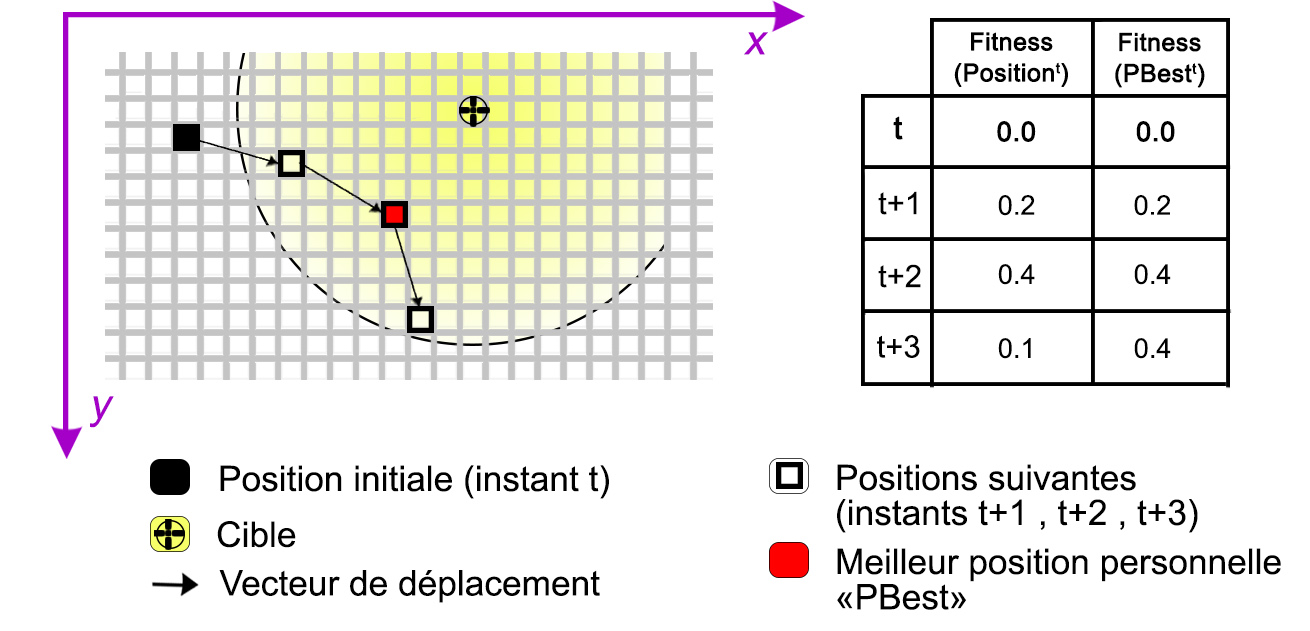
\includegraphics[width=0.9\textwidth]{PBest.jpg}%
	\vspace{-0.1 cm}
	\captionof{figure}{Représentation de la méthode de mise à jours du Pbest d'un éléphant.}\label{pbest}%
\end{center}


\textbf{Global best} (\label{Gbest}) ou encore meilleure position globale, est une position spécifique à l'essaim, c'est la meilleure position trouvée par tout l'essaim. 
%et par conséquent la plus proche par d'une certaine cible de tout l’essaim. 
On peut dire que le \textit{Gbest} consiste à trouver le max en termes de qualité des \textit{Pbest} de chaque éléphant, comme le montre l'équation suivante :

\begin{equation}
\begin{split}
Gbest= &(Gbest_{x},Gbest_{y})\\
Gbest^{t} = & \max(f(Pbest^{t}_{i}))
\end{split}
\end{equation}
Chaque éléphant a connaissance de la valeur du Gbest à chaque itération, c'est une connaissance commune à tous.

\subsection{Vélocité}
La vélocité combine la vitesse et la direction qui détermine la prochaine position de l'éléphant. La notation de la vélocité dans un environnement bidimensionnel est la suivante :
\begin{equation}
\begin{split}
V_{i,2}= & (v_{xi},v_{yi})\\
\end{split}
\end{equation}

\subsection{Mécanisme de déplacement}
\subsubsection{Mise à jour de la vélocité de l'éléphant}
La mise à jour de la vélocité est sujette à plusieurs paramètres dont les positions $Pbest$ et $Gbest$. Comme on peut le voir dans la figure \ref{velocity}, d'après la constante $p$ l'éléphant choisira de suivre sa meilleure position ou la meilleure du groupe, ce qui lui évite de stagner dans des optimums locaux.

\noindent
\begin{center}	  
	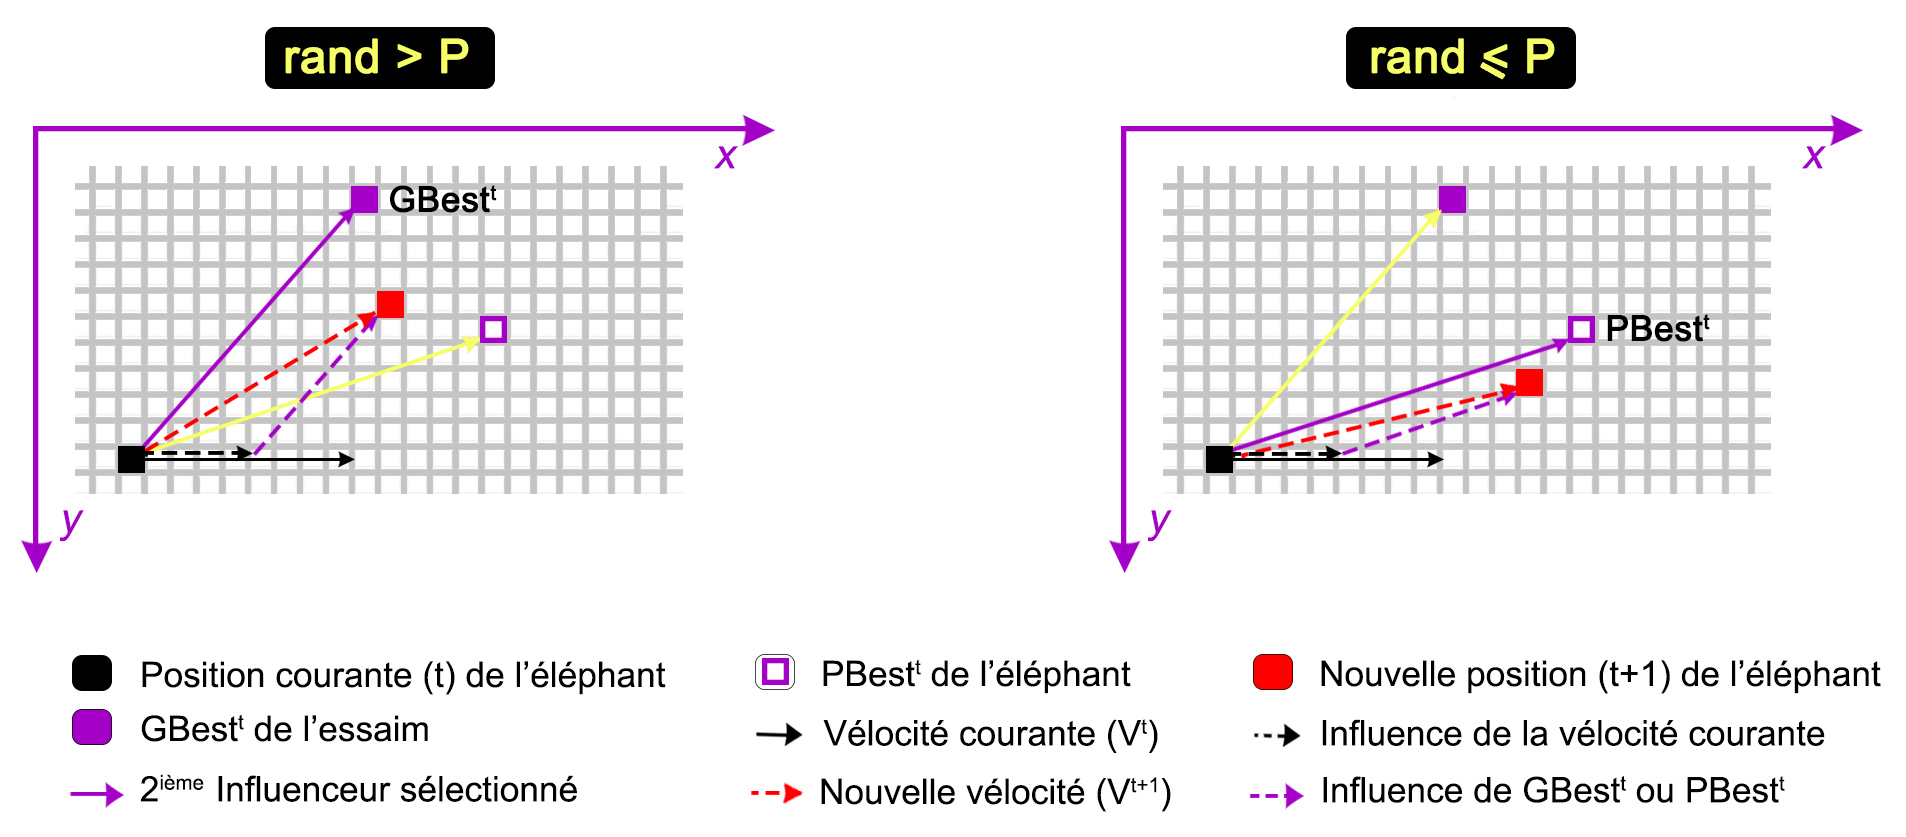
\includegraphics[width=1\textwidth]{deplacement-eswsa.jpg}%
	\vspace{-0.1 cm}
	\captionof{figure}{Représentation de la mise à jour de la vélocité d'un éléphant dans l'approche ESWSA.}\label{velocity}%
\end{center}

Vu qu'on se trouve dans un environnement bidimensionnel, on doit calculer deux vélocités, une selon les abscisses et une selon les ordonnées, ce processus est explicité dans les deux équations qui suivent:
%Le calcul de celle des abscisses se fait avec la première composante des positions $X_{i,2}$, $P_{best,i,2}$ , $G_{best,2}$, alors que celle des ordonnées se fait avec leur seconde composante. On explicite dans les deux équations qui suivent le calcul de la vélocité.
\begin{equation}
v_{xi}^{t+1}=
\left\lbrace
\begin{array}{ccc}
v_{xi}^{t} * w^t + rand * (Gbest_{x}^{t} - x_{i}^{t} ) & \mbox{si} & random > p\\
v_{xi}^{t} * w^t + rand * (Pbest_{xi}^{t} - x_{i}^{t} )  & \mbox{si} & random \leq p
\end{array}\right.
\end{equation}

\begin{equation}
v_{yi}^{t+1}=
\left\lbrace
\begin{array}{ccc}
v_{yi}^{t} * w^t + rand * (Gbest_{y}^{t} - y_{i}^{t} ) & \mbox{si} & random > p\\
v_{yi}^{t} * w^t + rand * (Pbest_{yi}^{t} - y_{i}^{t} )  & \mbox{si} & random \leq p
\end{array}\right.
\end{equation}
Notre environnement a des bornes fixes, cette formule de calcul risque de générer des vélocités trop grandes ce qui perturbe l'organisation et le comportement du groupe d'éléphants. Une solution est de borner la vélocité.
Soient les bornes de l'environnement représentées par le point $MaxP$
\begin{equation}
\begin{split}
MaxP= &(MaxP_{x},MaxP_{y})\\
v_{xi}^{t+1}=&v_{xi}^{t+1} \bmod MaxP_{x}\\
v_{yi}^{t+1}=&v_{yi}^{t+1} \bmod MaxP_{y}
\end{split}
\end{equation}






\subsubsection{Mise à jour de la position de l'éléphant}
Tout comme la \label{vélocité} la mise à jour de la position $X_{i,2}$ de l'éléphant $i$ se fait sur deux niveaux celui des abscisses et celui des ordonnées, l'équation de mise à jour est la suivante : 
\begin{equation}
\begin{split}
x_{i}^{t+1} & = v_{xi}^{t+1} + x_{i}^{t}\\
y_{i}^{t+1} & = v_{yi}^{t+1} + y_{i}^{t}
\end{split}
\end{equation}
Toujours pour éviter les valeurs aberrantes, on procède de la même manière qu'avec la vélocité en bornant la position, soit :
\begin{equation}
\begin{split}
MaxP= &(MaxP_{x},MaxP_{y})\\
x_{i}^{t+1}= & x_{i}^{t+1} \bmod MaxP_{x}\\
y_{i}^{t+1}= & y_{i}^{t+1} \bmod MaxP_{y}
\end{split}
\end{equation} 

Ainsi, la position de l'éléphant est calculée en tenant compte de sa connaissance de sa position à l'instant $t$ afin de calculer celle de l'instant $t+1$.





\subsubsection{Mise à jour de $W^t$ (poids d'inertie)}
Le poids d'inertie est un paramètre qui influence la vélocité et ainsi le calcul des positions des éléphants. Comme on a pu le voir dans le chapitre 2  section ~\ref{LDIW} page ~\pageref{LDIW}, l'équation choisie calcule le poids d'inertie selon le nombre d'itérations $t$
avec l'initialisation suivante :
\begin{equation}
\begin{split}
W_{max}= & 0.9\\
W_{min}= & 0.1\\
t_{max}= & 1000\\
W^{t} = & W_{max} - \frac{W_{max} - W_{min}}{t_{max}} * t
\end{split}
\end{equation}
$W^t$ joue un rôle important dans la convergence des éléphants vers la solution optimale, il détermine le taux de vélocité mémoire. C'est-à-dire la vélocité à l'instant $t$, qui influencera la prochaine vélocité à l'instant $t+1$.
Il permet alors de contrôler et varier la vitesse et la trajectoire afin d'explorer au mieux l'environnement de recherche.\\






\section{Fonctionnement d'ESWSA}
Dans ESWSA, chaque éléphant se comporte comme un robot indépendant du groupe mais coopératif. Doté d'une mémoire qui se présente en sa $pbest$ et $gbest$ qui sont nécessaires pour le choix des trajectoires possibles. L'organisation des éléphants lors de la recherche suit un schéma dont on explicite les étapes dans la figure \ref{eswsa} et dans le processus suivant :



\subsection{Initialisation}
Comme toute méta-heuristique, ESWSA commence par une étape d'initialisation déterminante pour le bon déroulement de la recherche à savoir :
\subsubsection{Paramètres empiriques}
Initialiser les paramètres empiriques consiste à leur choisir des valeurs fixes. Ils sont souvent le sujet d'un réglage pour augmenter l'efficacité et performance des approches basées essaim. Les paramètres d'ESWSA sont : 
\textit{Tmax, nbrEle, P, $W^t$, MaxP, MinP.}

\subsubsection{Positions initiales des éléphants}
L'emplacement initial des éléphants est aussi un facteur influent de la recherche. On initialise chaque éléphant à une position aléatoire en respectant les contraintes énoncées dans le chapitre 3.

\subsubsection{Pbest pour chaque éléphant}
Après avoir choisi les positions des éléphants, on doit évaluer la qualité de cette position. Cette évaluation permet d'initialiser les $Pbest$ (Meilleure position personnelle en termes de qualité) de chaque éléphant de l'essaim.

\subsubsection{Gbest}
Comme on a pu l'expliquer plus haut dans \ref{Gbest}, la position \textit{Gbest} (Meilleure position globale de tout l'essaim) est initialisée selon le maximum des positions $pbest$ évaluées en termes de qualité. En d'autres termes, celle qui détient la valeur maximum de la fonction objectif.

Une fois les initialisations faites, le processus d'ESWSA se met en marche selon ce qui suit :

\subsection{Mise à jour de la vélocité pour chaque éléphant}
Chaque éléphant de l'essaim se voit mettre à jour sa vélocité, cela se fait avec \textit{le choix d'un nombre aléatoire} qui détermine l'équation à choisir. Si ce nombre aléatoire est inférieur au paramètre empirique \textit{p} alors la vélocité sera calculée par rapport à sa position $Pbest$, sinon ça sera d'après le $Gbest$. Autrement dit l'éléphant choisira de privilégier le suivi de sa position $Pbest$ ou bien $Gbest$ à chaque itération.

\subsection{Calcul de la prochaine position de chaque éléphant}
Une fois la vélocité calculée, elle nous permet de mettre à jour la position de chaque éléphant selon l'équation de mise à jour voir section \ref{vélocité}.
%, en additionnant la vélocité à la position précédente de l'éléphant.

\subsection{Déplacement des robots}
Vu qu'un éléphant simule un robot, son déplacement se fait en employant la stratégie d'évitement d'obstacles, en cas d'environnement à obstacles.

\subsection{Évaluation des positions des éléphants}
Un éléphant a un angle de vue lui permettant de voir autour de lui sur une superficie de dix cases, ces cases seront évaluées selon la fonction objectif. L'éléphant gardera la position de la meilleure case.

Si une cible est détecté, le nombre de cibles trouvées \textit{"c"} est alors incrémenté.

\subsection{Mise à jour du Pbest de chaque éléphant}
Pendant la recherche, la position $Pbest$ est susceptible de changer, c'est pourquoi après chaque évaluation un test est effectué pour savoir si la mise à jour du $Pbest$ de l'éléphant est nécessaire. Ça signifie qu'on a trouvé une meilleure position nous rapprochons d'une cible.

\subsection{Mise à jour de Gbest}
Après l'éventuelle mise à jour des positions $Pbest$, vient la mise à jour de la position $Gbest$, où un test est effectué également pour un potentiel changement du $Gbest$.

\subsection{Mise à jour du $W^t$ (poids d'inertie)}
Le poids d'inertie est relatif à chaque itération dont on calcule la valeur selon l'itération courante.

\subsection{Critère d'arrêt de la recherche}
Le processus d'ESWSA s'exécute en boucle, en incrémentant le nombre d'itérations \textit{"t"},  jusqu'à la rencontre de toutes les \textbf{"nbrCible"} cibles ou bien jusqu'à atteindre le nombre maximum d'itérations \textbf{"MaxIter"}. 


\noindent
\begin{center}	  
	\captionsetup{width=1\linewidth}
	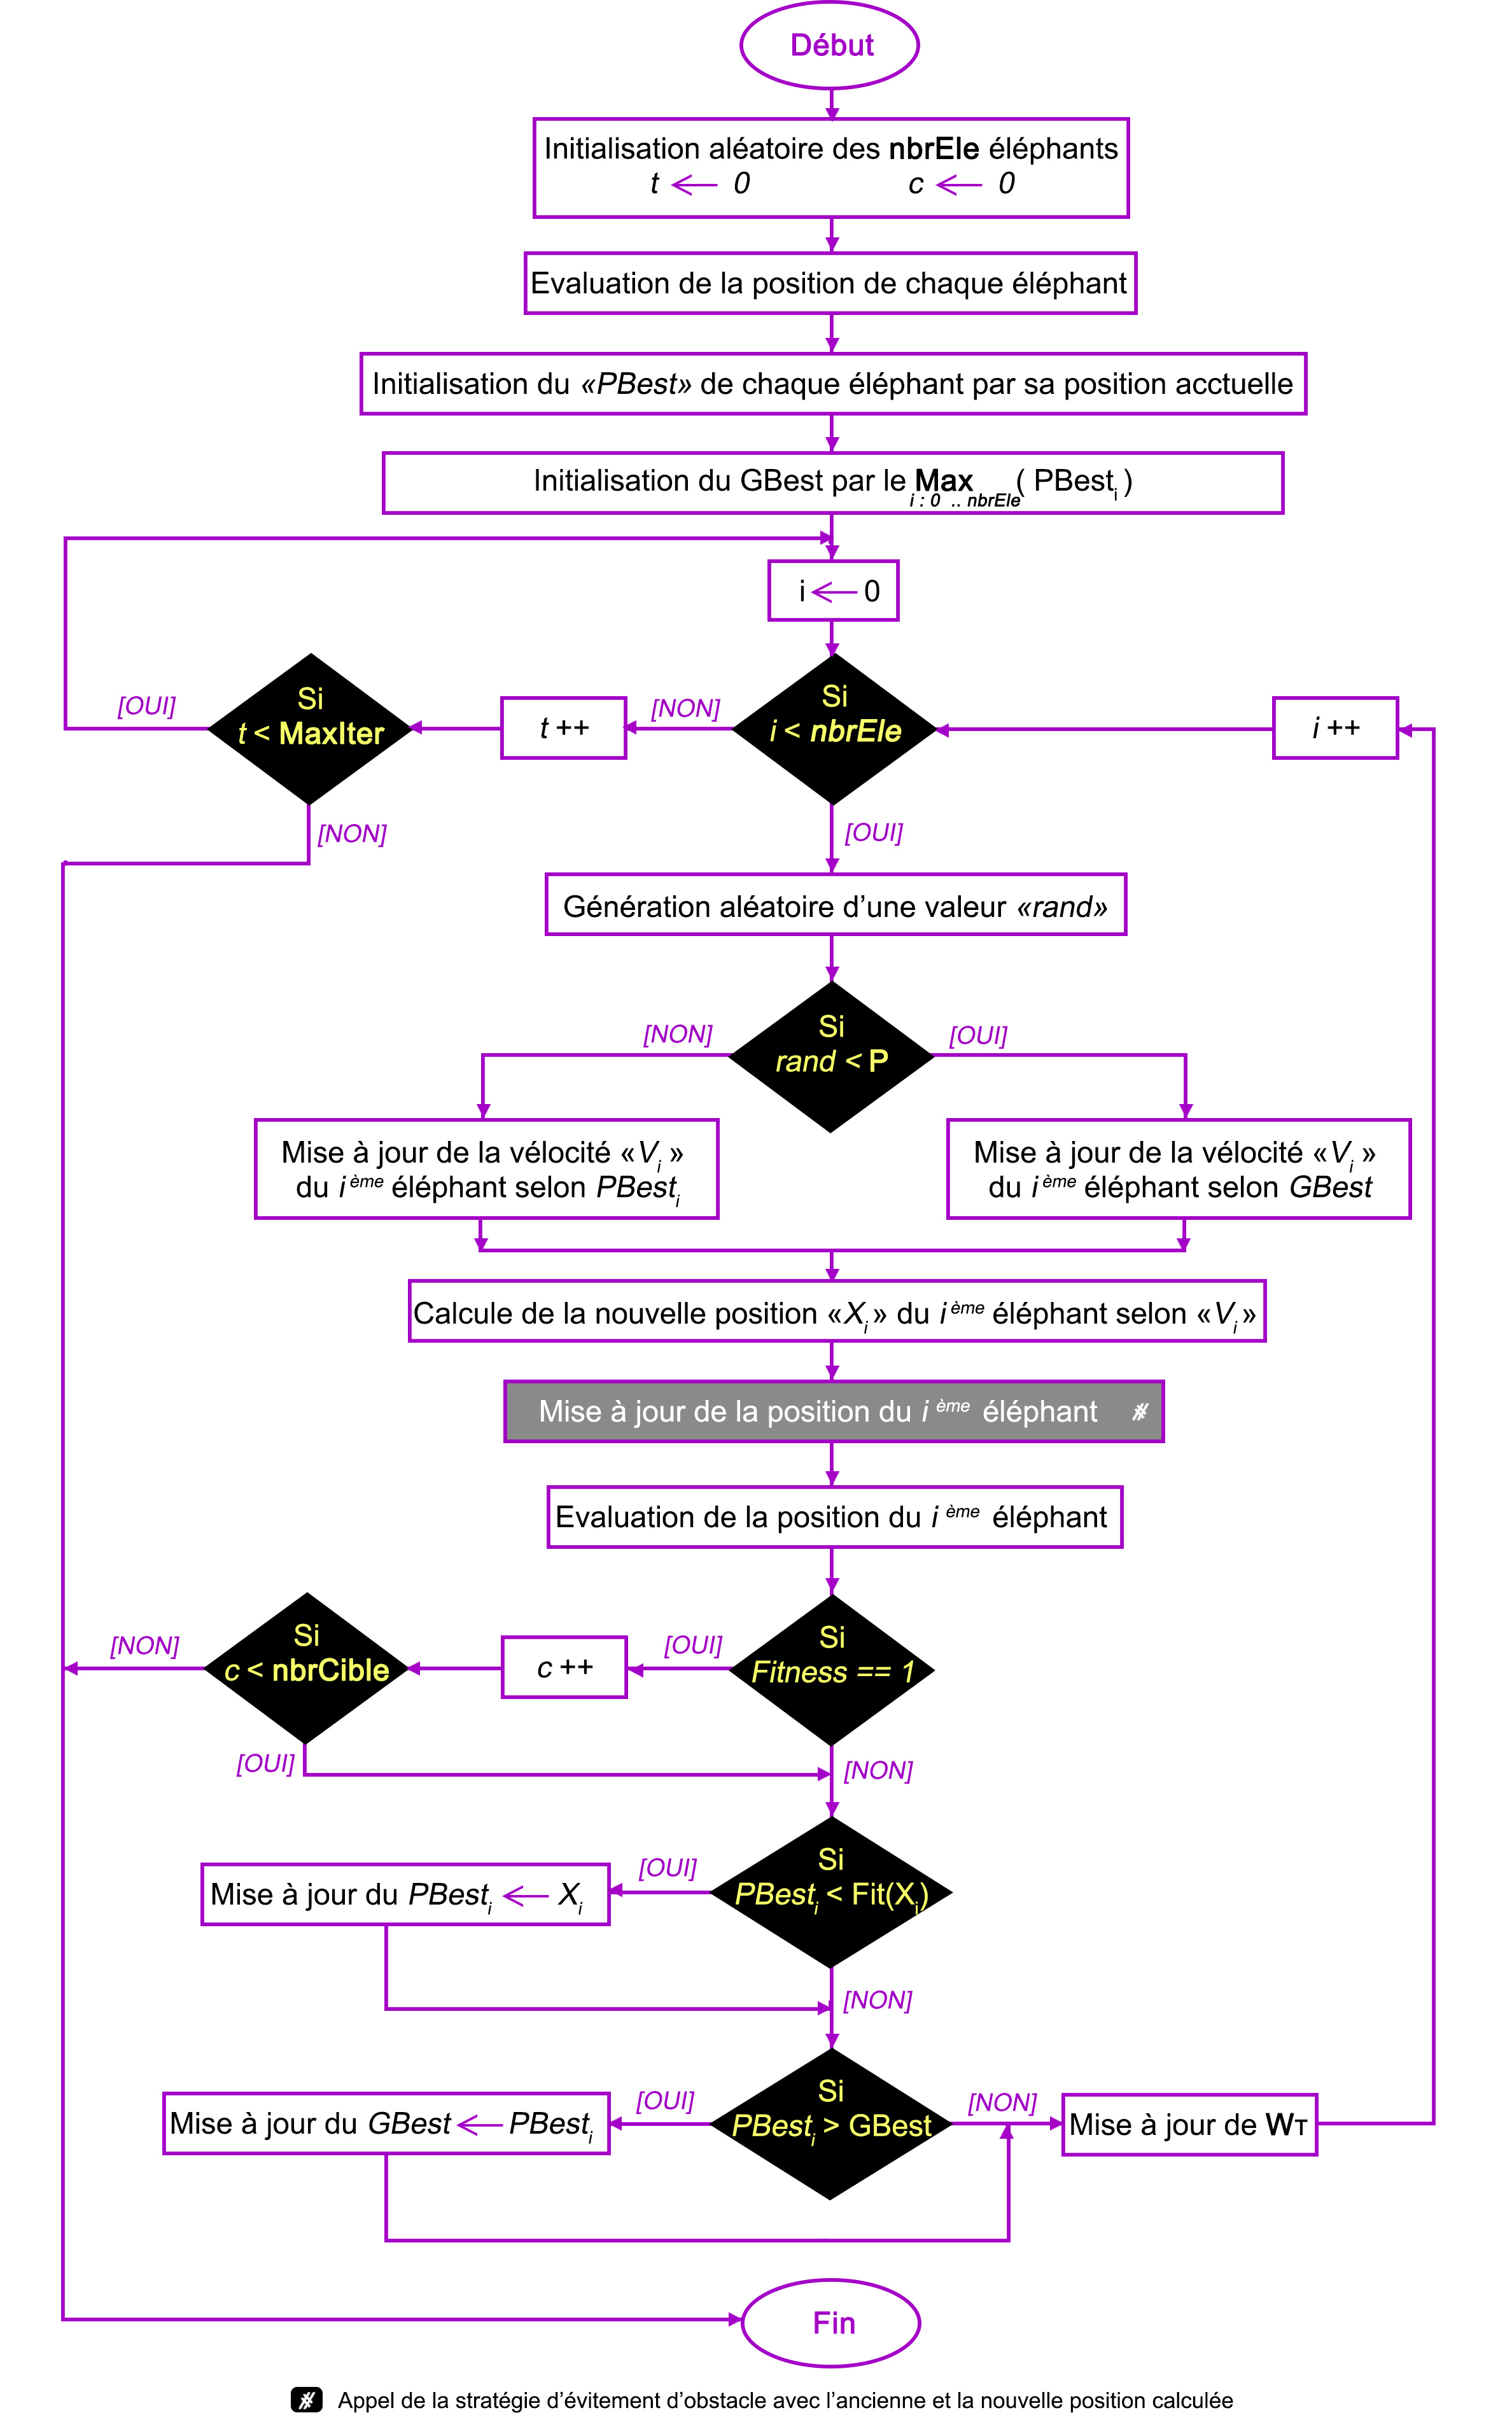
\includegraphics[width=0.8\textwidth]{eswsa.jpg}%
	\vspace{-0.3cm}
	\captionof{figure}{Organigramme du mode de fonctionnement de l'approche ESWSA.}\label{eswsa}%
\end{center}







\section{Conclusion}
Les deux algorithmes présentés reposent sur le comportement des éléphants, mais vus sous deux angles bien différents. C'est pourquoi leur fonctionnement n'a rien en commun, exploitant chacun un aspect différent relatif aux éléphants et groupes d'éléphants.
Le dernier chapitre sera consacré à la réalisation et expérimentations de toutes les approches citées dans ce chapitre et celui qui le précède.

